\subsection{Tool System}
\label{sec:tool_system}

The tools through which the agent interacts with the development environment form an extensible ecosystem that balances comprehensive capability with context efficiency, safety with flexibility, and built-in tools with dynamic discovery. \Cref{tab:full_tools} in \Cref{app:tools} provides a complete catalog of all 35 built-in tools; the remainder of this section describes the registry architecture that organizes them into handler categories, then details each category: file operations, shell execution, web interaction, semantic code analysis via LSP, user interaction and task management, external tool discovery via MCP, and subagent delegation. A defense-in-depth safety architecture spans all categories.

\subsubsection{Registry Architecture and Schema Construction}
\label{sec:tool_registry}

A flat namespace of tools becomes unmanageable as capabilities grow: hard-coded dispatch logic is inflexible, and dynamic plugin loading without structure is unsafe. Alternatives range from hardcoded tool sets (simple but cannot add capabilities without code changes) to flat dynamic loading (flexible but chaotic, leading to namespace collisions, lack of organization, and difficult safety management). \name adopts a registry with handler categories, organizing tools into handler classes with schema-based registration.

\paragraph{Three separated concerns.} \Cref{fig:tool_system} illustrates the architecture. The tool system separates schema construction, dispatch routing, and lifecycle hooks into distinct components.

\begin{figure}[htbp]
    \centering
    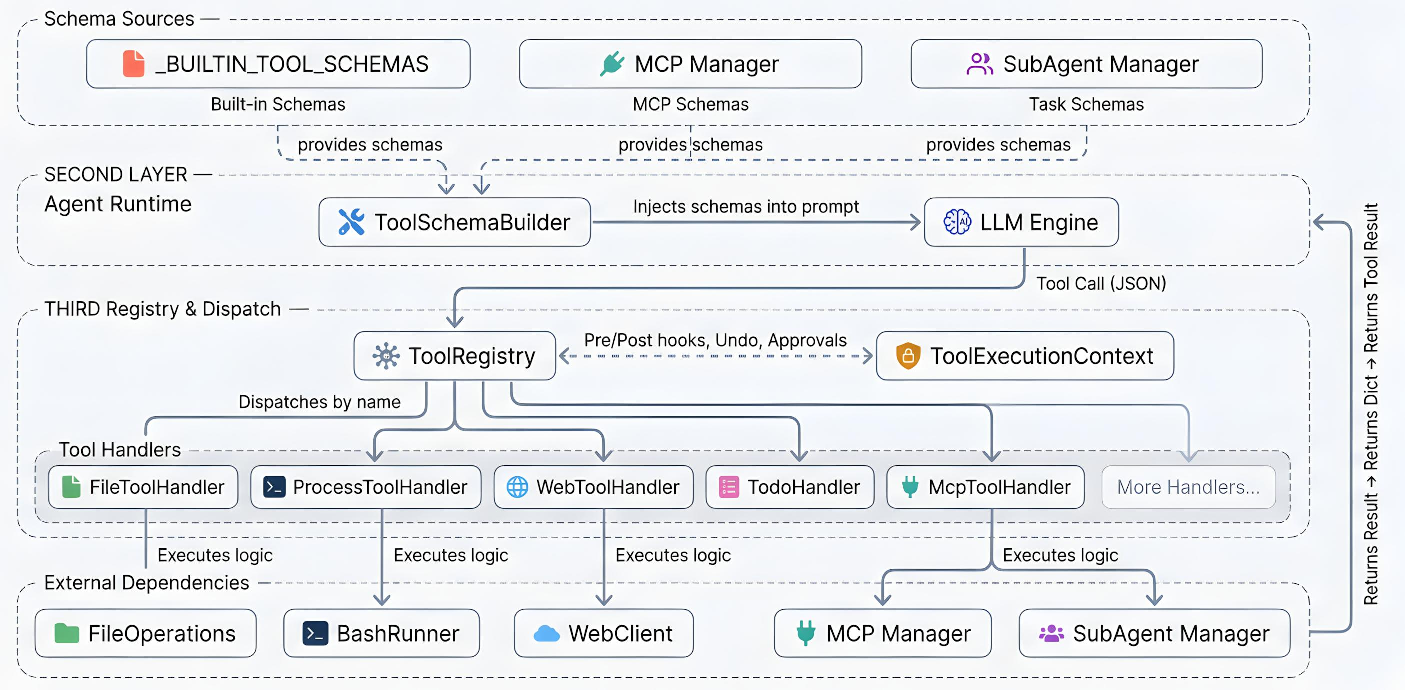
\includegraphics[width=\linewidth]{figures/tool_system.pdf}
    \caption{Expanded view of the Tool layer from \Cref{fig:architecture}. \textbf{ToolSchemaBuilder} assembles JSON schemas from three sources (static built-in definitions, dynamically discovered MCP tools, subagent schemas) and injects them into the LLM prompt. \textbf{ToolRegistry} dispatches tool calls to category-based handlers, each receiving a \texttt{ToolExecutionContext} with cross-cutting services. Pre/post lifecycle hooks intercept calls for safety enforcement and extensibility.}
    \label{fig:tool_system}
\end{figure}

\textbf{ToolSchemaBuilder} assembles JSON schemas from three sources: (1)~static \texttt{\_BUILTIN\_TOOL\_SCHEMAS} defining approximately 40 built-in tools, with descriptions loaded from markdown templates via \texttt{load\_tool\_description()}; (2)~dynamically discovered MCP schemas, including only those tools in the \texttt{\_discovered\_mcp\_tools} set to avoid context bloat; and (3)~subagent schemas injected by the \texttt{SubAgentManager} when present. The assembled schemas are injected into the LLM prompt, giving the model awareness of available capabilities.

\textbf{ToolRegistry} serves as the central dispatcher, mapping tool names to handler methods across 12 handler classes organized by category (file, process, web, notebook, user interaction, task management, thinking, MCP discovery, batch execution; see \Cref{tab:full_tools} in \Cref{app:tools} for the complete mapping). Each handler receives a \texttt{ToolExecutionContext} that bundles cross-cutting services: mode manager, approval manager, undo manager, task monitor, session manager, UI callback, and file-time tracker. The registry enforces mode restrictions by blocking write operations in plan mode with informative errors before dispatching to handlers.

\textbf{Lifecycle hooks} provide extensibility without modifying handler code. The hook system defines ten lifecycle events (\texttt{SESSION\_START}, \texttt{USER\_PROMPT\_SUBMIT}, \texttt{PRE\_TOOL\_USE}, \texttt{POST\_TOOL\_USE}, \texttt{POST\_TOOL\_USE\_FAILURE}, \texttt{SUBAGENT\_START}, \texttt{SUBAGENT\_STOP}, \texttt{PRE\_COMPACT}, \texttt{SESSION\_END}, and \texttt{STOP}) covering the full agent lifecycle from session initialization to shutdown. \texttt{PreToolUse} hooks fire synchronously before execution: a hook returning exit code~2 hard-blocks the tool call, returning an error to the model that no amount of prompt engineering or approval configuration can override. Hooks can also mutate tool arguments by returning a JSON object with an \texttt{updatedInput} field, enabling transparent command rewriting (e.g., injecting \texttt{-{}-dry-run} flags). \texttt{PostToolUse} and \texttt{PostToolUseFailure} hooks fire asynchronously via a thread pool after execution, suitable for auditing and logging without delaying the agent. External scripts registered as hooks receive full event context as JSON on stdin (including session ID, working directory, tool name, tool input, and (for post-hooks) tool response), enabling project-specific policies such as blocking writes to protected paths, enforcing naming conventions, or streaming audit logs to external systems. Hook matchers use compiled regex patterns against tool names, allowing fine-grained targeting from single-tool rules to catch-all policies.

\paragraph{Design evolution.} Early versions registered tools directly in a global namespace, causing naming collisions and complex per-tool safety configuration. Category-based handlers solved both: safety rules apply at the category level, and each category provides implicit namespacing.

\paragraph{Runtime approval.}
\label{sec:approval}
Before any tool call reaches its handler, the runtime approval system gates execution based on user-configured trust boundaries. Three autonomy levels control the default posture: \emph{Manual} requires explicit approval for every tool call; \emph{Semi-Auto} auto-approves read-only operations (a curated allowlist of commands such as \texttt{ls}, \texttt{cat}, \texttt{git status}) while prompting for writes; and \emph{Auto} approves all operations for trusted workflows. Beyond the default level, an \texttt{ApprovalRulesManager} evaluates each command against a prioritized rule set with four rule types: \textsc{Pattern} (regex match against the full command string), \textsc{Command} (exact match), \textsc{Prefix} (prefix match, e.g., \texttt{git} matching \texttt{git push}), and \textsc{Danger} (regex match with auto-deny semantics). Default danger rules at priority~100 (matching patterns such as \texttt{rm -rf /}, \texttt{rm -rf *}, and \texttt{chmod 777}) are always active and cannot be overridden by user configuration or approval-level changes. Rules are evaluated in priority order; the first match determines the action (auto-approve, auto-deny, require approval, or require the user to edit the command before execution).

Approval rules persist across sessions via two JSON stores: user-global rules at \texttt{\~{}/.opendev/permissions.json} and project-scoped rules at \texttt{.opendev/permissions.json}. When both exist, project rules take priority for the same pattern, enabling per-repository trust boundaries (e.g., a shared project can restrict \texttt{docker} commands that a user's personal config allows). The approval flow adapts to the active frontend: the TUI presents a blocking \texttt{prompt\_toolkit} menu with keyboard navigation, while the Web~UI broadcasts an \texttt{approval\_required} WebSocket event and polls a threading event with a 300-second timeout, rendering an approval dialog in the browser. Every approval decision (command, action taken, matching rule, and timestamp) is recorded in a \texttt{CommandHistory} for audit.

\subsubsection{File Operations}
\label{sec:file_ops}

Five tools handle all file-system interactions (see File Ops category in \Cref{tab:full_tools}), from reading and writing to structured editing and searching. Together they form the agent's primary means of code manipulation.

\paragraph{\texttt{read\_file}: Line-numbered file reading.} Reads file contents with \texttt{cat -n} style line numbering, providing the agent with precise positional references for subsequent edits. Three parameters control the read window: \texttt{file\_path} (required), \texttt{offset} (1-based line start, default 1), and \texttt{max\_lines} (default 2000). The handler applies several output transformations before returning content to the agent:

\begin{packeditemize}
\item \textbf{Binary detection:} Non-text files are detected and rejected with descriptive errors rather than returning corrupted byte sequences.
\item \textbf{Output truncation:} Content exceeding 30,000 characters is truncated using a head-tail strategy that preserves the first 10,000 and last 10,000 characters with a truncation marker between them. This ensures the agent sees both the beginning (imports, class declarations) and end (recent additions) of long files.
\item \textbf{Per-line truncation:} Individual lines exceeding 2,000 characters are truncated to prevent minified code or data files from consuming excessive context.
\item \textbf{Stale-read tracking:} A \texttt{FileTimeTracker} records the timestamp of each read. The tracker records \texttt{datetime.now()} keyed by \texttt{(session\_id, file\_path)} on every successful read. Before any edit, \texttt{assert\_fresh()} verifies that \texttt{os.path.getmtime(file\_path)} $\leq$ \texttt{read\_time + 50ms}, where the 50ms tolerance accommodates filesystem timestamp granularity (FAT32 rounds to 2-second boundaries; NTFS and ext4 offer sub-millisecond precision, but network filesystems introduce jitter). If the assertion fails, the edit is rejected with an error instructing the agent to re-read the file, preventing silent overwrites of concurrent user edits. A \texttt{threading.Lock} per file path serializes concurrent write attempts to the same file.
\end{packeditemize}

\paragraph{\texttt{write\_file}: New file creation.} Creates new files only by rejecting attempts to overwrite existing files, directing the agent to use \texttt{edit\_file} instead. This constraint prevents accidental full-file overwrites, which are a common failure mode when agents reconstruct files from memory rather than applying targeted edits. Parameters: \texttt{file\_path}, \texttt{content}, and \texttt{create\_dirs} (which auto-creates parent directories when set). The handler runs the approval workflow for write operations, records the action with the undo manager for rollback capability, and returns the file path and byte count on success.

\paragraph{\texttt{edit\_file}: 9-pass fuzzy matching.} When an LLM-based agent edits a file, it specifies \texttt{old\_content} to find and \texttt{new\_content} to replace. In practice, the LLM frequently produces \texttt{old\_content} that differs slightly from the actual file: trailing whitespace variations, indentation mismatches, escape sequence differences, or minor reformatting from reconstructing code from memory rather than verbatim copy. A strict exact-match edit tool fails on these cases, producing ``content not found'' errors that consume context with error messages and recovery attempts.

The edit tool implements a chain-of-responsibility pattern with nine replacer classes, each addressing a specific mismatch category, from exact match through whitespace normalization, indentation flexibility, escape handling, and context-aware anchor matching (\Cref{app:fuzzy} enumerates all nine passes with descriptions). Each replacer returns the \emph{actual substring found in the original file} (not the search query), so the replacement preserves the file's original formatting. Debug logging records which pass succeeded. The chain short-circuits on first match, so exact matches incur zero overhead from the fuzzy passes.

Beyond matching, the edit handler enforces several safety and observability measures. Stale-read validation rejects edits to files modified since the agent's last read. Uniqueness verification ensures the match is unambiguous: multiple matches produce errors rather than silent mis-edits. Backup state is created for undo tracking. After a successful edit, the handler calls \texttt{lsp.touch\_file(filepath)} to notify the running language server of the change, then waits up to 3 seconds (debounced) for diagnostics. Only Error-severity diagnostics are included; warnings and hints are suppressed to avoid context noise. Up to 20 diagnostics are appended to the tool output as structured feedback (e.g., ``\texttt{LSP errors detected: line 42: undefined variable `foo'}''), giving the agent immediate feedback and enabling self-correction in the same turn. If no LSP server is running for the file type, the check is silently skipped. A unified diff is generated for display to the user.

\paragraph{\texttt{list\_files}: Directory listing and glob search.} Lists directory contents or performs glob-based file search. Parameters: \texttt{path} (directory to list), \texttt{pattern} (glob expression for filtering), \texttt{max\_results} (default 100). Results render as a tree display showing directory structure. Common ignore patterns are excluded by default: \texttt{node\_modules}, \texttt{.git}, \texttt{\_\_pycache\_\_}, \texttt{.venv}, \texttt{.DS\_Store}, and other platform-specific artifacts. Output is capped at 500 entries to prevent context overflow from large repositories.

\paragraph{\texttt{search}: Dual-mode content search.} Supports two search modes addressing complementary needs. With \texttt{type="text"}, the tool delegates to ripgrep for high-performance regex-based content search with configurable context lines, supporting the full PCRE2 pattern syntax. With \texttt{type="ast"}, the tool delegates to ast-grep for structural code search using language-aware pattern templates with \texttt{\$VAR} wildcards (e.g., \texttt{if \$COND: \$BODY} matches any Python if-statement regardless of specific condition or body content). Parameters: \texttt{pattern} (regex or ast-grep template), \texttt{path} (search root), \texttt{type} (``text'' or ``ast''), \texttt{lang} (language hint for ast mode). Results are capped at 50 matches and 30,000 characters total output.

\paragraph{Design evolution.} The initial edit tool used a two-pass strategy (exact match, then whitespace-stripped match). This was the single largest source of ``content not found'' errors. Analyzing failure logs revealed that LLM formatting drift falls into distinct, predictable categories (whitespace normalization, indentation shifts, escape sequence differences, partial-context anchoring), each addressable by a targeted matching pass. Generalizing this observation into a chain-of-responsibility architecture with nine progressively relaxed replacers resolved the vast majority of edit failures while preserving exact-match performance through short-circuit evaluation.

\subsubsection{Shell Execution and Background Tasks}
\label{sec:bash_tool}

Four tools handle shell execution and background task management (see Process category in \Cref{tab:full_tools}). The agent needs to run arbitrary shell commands for testing, building, and system interaction, but must do so safely; long-running processes like development servers require background execution with output capture.

\begin{figure}[htbp]
    \centering
    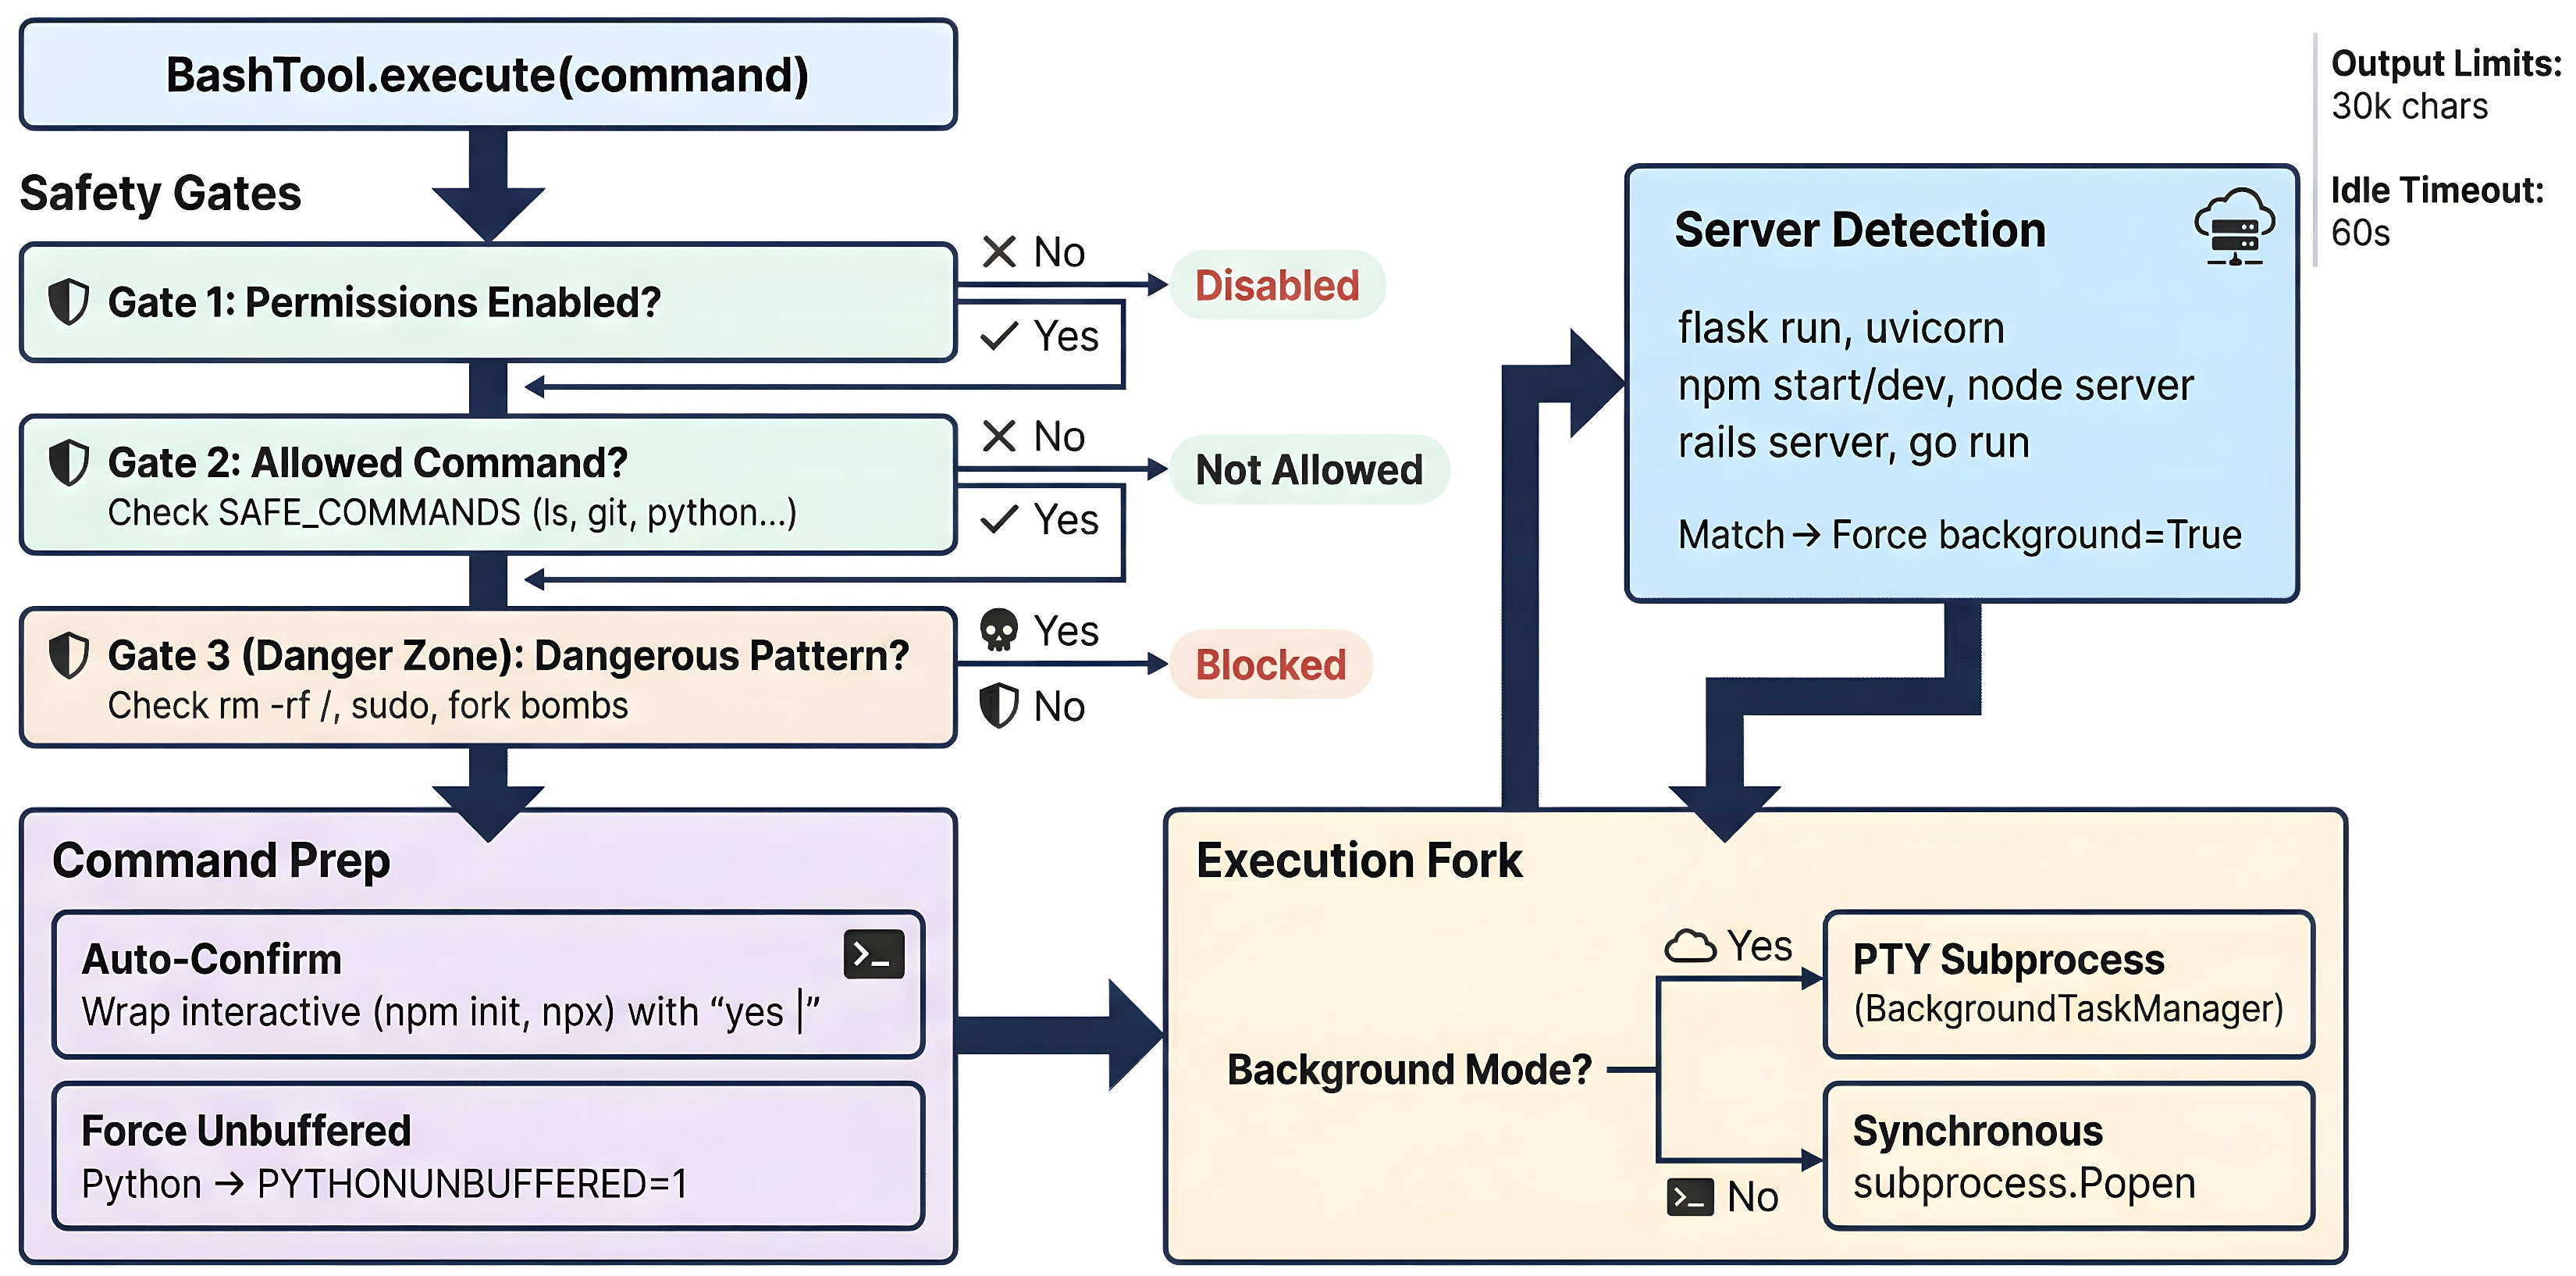
\includegraphics[width=\linewidth]{figures/bash_tool.pdf}
    \caption{Detailed pipeline for the Process handler (\Cref{fig:tool_system}). Commands pass through three safety gates (permission config, allowed-command matching, dangerous pattern blocking), then command preparation (auto-confirm, unbuffered Python), server detection (regex match against 16 patterns for auto-background promotion), execution fork (PTY-based background or piped foreground with process-group isolation), output management (30k char limit with head/tail truncation, 100ms polling), and timeout/interrupt handling (60s idle, 600s absolute, \texttt{InterruptToken} integration).}
    \label{fig:bash_tool}
\end{figure}

\paragraph{\texttt{run\_command}: Six-stage shell execution.} \Cref{fig:bash_tool} illustrates the pipeline, which processes every shell command through six stages: (1)~safety gates that block dangerous patterns with no override, (2)~command preparation that auto-confirms package manager prompts and unbuffers Python output, (3)~server detection via regex match against 16 framework patterns (\Cref{app:server_patterns}) that auto-promotes long-running servers to background mode, (4)~execution fork between PTY-based background and piped foreground with process-group isolation, (5)~output management with 30k-character head-tail truncation and 100ms polling, and (6)~timeout handling with 60-second idle and 600-second absolute limits. \Cref{app:bash} provides the full stage-by-stage details and the complete server pattern table.

Commands promoted to background are registered with the \texttt{BackgroundTaskManager}, which assigns 7-character hex IDs (from \texttt{uuid4().hex[:7]}, providing ${\sim}268$M unique values). Registration creates the task record, opens an output file at \texttt{/tmp/opendev/\{sanitized-dir\}/tasks/\{id\}.output}, writes any initial startup output captured during the first 20 seconds, and spawns a daemon thread that continuously streams PTY output to the file via \texttt{select.select()} polling. Tasks transition through four states: RUNNING $\to$ COMPLETED (exit code 0), FAILED (non-zero exit), or KILLED (via signal). Listener callbacks notify the UI of each state transition, enabling real-time status display in the TUI footer.

\paragraph{\texttt{list\_processes}: Background task listing.} Returns all tracked background tasks with PID, status (running/completed/failed/killed), and wall-clock runtime. This gives the agent visibility into what processes are active, enabling it to check on long-running servers, identify stalled builds, or determine which tasks need attention.

\paragraph{\texttt{get\_process\_output}: Task output retrieval.} Retrieves the last 100 lines from a background task's output file by task ID, giving the agent access to server logs, build output, and error messages without needing to re-run the command. This is essential for monitoring development servers, inspecting test results from background runs, and diagnosing failures in long-running processes.

\paragraph{\texttt{kill\_process}: Graceful process termination.} Terminates a running background task using graceful escalation: send SIGTERM to the entire process group via \texttt{os.killpg()}, wait 5 seconds for graceful shutdown, then escalate to SIGKILL if the process is still running. The daemon output thread is signaled to stop, and the PTY master file descriptor is closed. Process group killing ensures that child processes spawned by the command (e.g., webpack dev server spawning file watchers) are terminated along with the parent.

\paragraph{Design evolution.} The initial implementation used \texttt{subprocess.run()} with a fixed timeout. Development servers invariably hit the timeout and were killed. Activity-based idle timeout solved the server problem, and PTY-based execution solved output buffering issues where programs would produce no visible output until process termination.

\subsubsection{Web Interaction}
\label{sec:web_tools}

Four tools provide web interaction capabilities (see Web category in \Cref{tab:full_tools}) for documentation research, content inspection, and browser-based testing. All web tools are read-only and safe for use in plan mode.

\paragraph{\texttt{fetch\_url}: Browser-engine web fetching.} Retrieves web content using Crawl4AI, a browser-engine crawling library built on Playwright. The browser-engine approach handles JavaScript-rendered content that simple HTTP clients would miss (single-page applications, dynamically loaded documentation). HTML is converted to markdown for context-efficient consumption by the LLM. Output is capped at 50,000 characters with a 30-second per-page timeout. File downloads are blocked to prevent disk abuse.

For multi-page exploration, the tool supports deep crawling with three configurable strategies: breadth-first (BFS), depth-first (DFS), or best-first (priority by content relevance). Parameters control maximum crawl depth, page limit, and domain filters to prevent crawling beyond the target site. Playwright Chromium is auto-installed on first use, with the installation triggered transparently when the tool is first invoked.

\paragraph{\texttt{web\_search}: Privacy-respecting search.} Searches the web via DuckDuckGo, chosen for its privacy-respecting design (no user tracking or search history retention). Returns up to 10 results, each containing title, URL, and text snippet. Domain filters allow restricting results to specific sites (e.g., searching only official documentation domains). The tool returns structured results that the agent can then follow up on with \texttt{fetch\_url} for full content retrieval.

\paragraph{\texttt{capture\_web\_screenshot}: Visual page capture.} Takes full-page screenshots via Playwright's headless browser. Configurable viewport dimensions (default 1920$\times$1080) allow capturing pages at different responsive breakpoints. Optional PDF output mode produces paginated documents. Timeout extends up to 180 seconds for complex pages with heavy JavaScript initialization. Returns the screenshot file path, which the agent can reference in subsequent analysis or present to the user.

\paragraph{\texttt{open\_browser}: System browser launch.} Opens a URL or local file in the system's default browser via platform-native commands. Local file paths are automatically converted to \texttt{file://} URIs. This tool bridges the gap between the agent's headless environment and the user's visual workflow, making it useful for previewing generated HTML, reviewing web applications under development, or opening documentation links that require authentication the agent cannot provide.

\paragraph{Design evolution.} The initial implementation used simple HTTP requests via the \texttt{requests} library, which failed on JavaScript-rendered single-page applications that dominate modern documentation and web frameworks. Switching to Crawl4AI with Playwright's browser engine solved this, enabling full DOM rendering before content extraction.

\subsubsection{Multi-Language Semantic Code Analysis via LSP}
\label{sec:lsp}

Six tools provide multi-language semantic code analysis via LSP (see Symbols category in \Cref{tab:full_tools}), split into two read-only navigation tools and four structural editing tools. Text-based tools can search for strings but miss semantic structure: finding all usages of a method requires distinguishing method calls from variable names, handling overloading, and tracking references across files. Building custom parsers for each language is infeasible, so \name adopts Language Server Protocol integration via standard language servers~\cite{microsoft2016lsp}, reusing a mature ecosystem where each server is maintained by domain experts.

\begin{figure}[htbp]
    \centering
    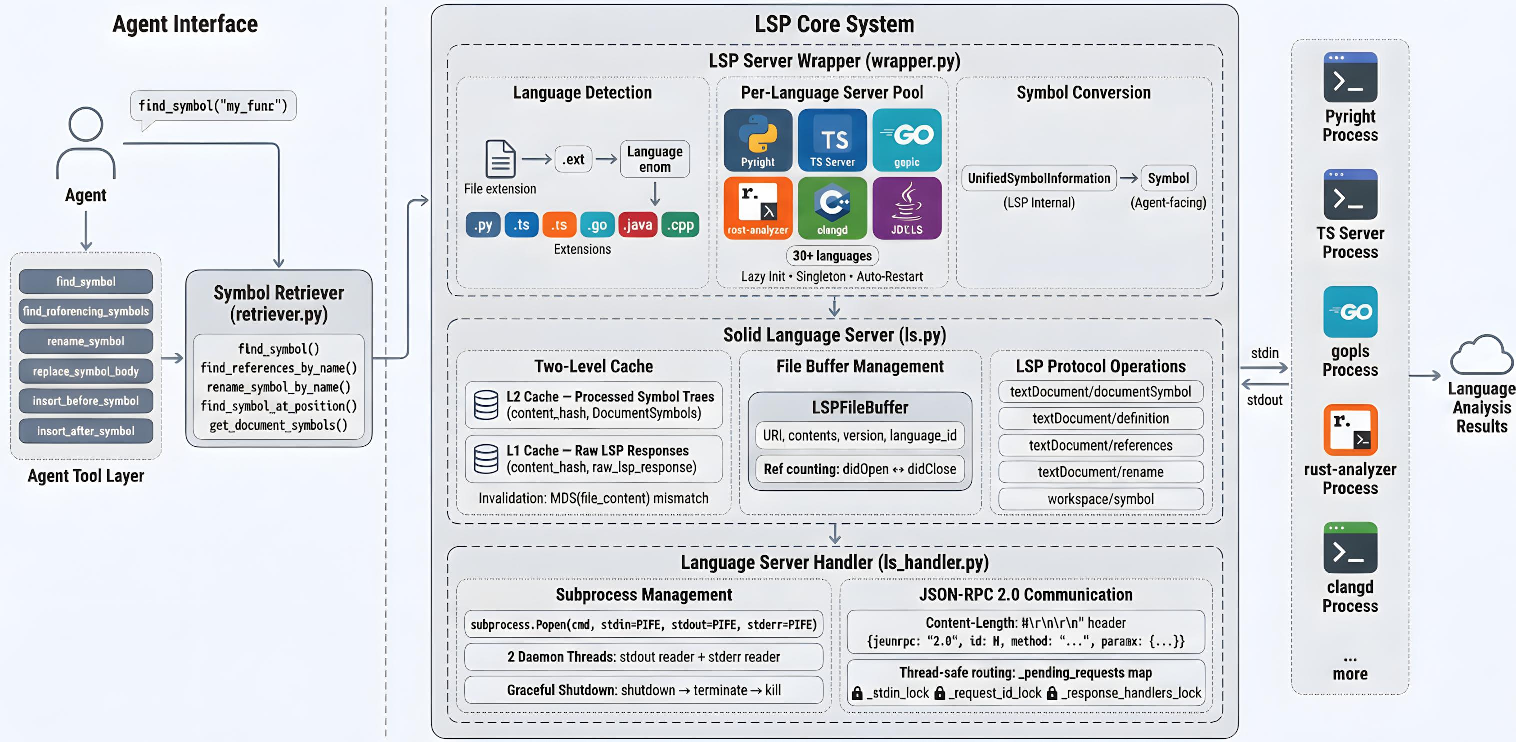
\includegraphics[width=\linewidth]{figures/lsp.pdf}
    \caption{Detailed architecture for the Symbols handler (\Cref{fig:tool_system}). The system is organized into four layers: Agent Tool Layer (six symbol tools), Symbol Retriever (unified API), LSP Server Wrapper (language detection, per-language server pool, symbol conversion), and Solid Language Server (two-level cache, file buffer management, LSP protocol operations). The Language Server Handler manages subprocess lifecycle and JSON-RPC~2.0 communication with external language server processes. Language detection maps 30+ file extensions to their respective servers, which are started lazily on first query and reused across subsequent requests.}
    \label{fig:lsp}
\end{figure}

\paragraph{Four-layer LSP abstraction.} \Cref{fig:lsp} illustrates the architecture, organized into four layers that progressively translate between agent-facing tool calls and language-server-specific protocol messages. The \emph{Agent Tool Layer} exposes the six tools described below; each accepts a file path and a symbol name, with language detection, server selection, and protocol translation handled transparently by the lower layers. The \emph{Symbol Retriever} provides a unified API that resolves symbol names to positions using a \texttt{NamePathMatcher} supporting exact match (\texttt{MyClass.method}), partial path match (\texttt{method} matching any symbol whose path ends with \texttt{.method}), and wildcard match (\texttt{My*} matching \texttt{MyClass}, \texttt{MyModule}). The \emph{LSP Server Wrapper} handles language detection (30+ file extensions; see \Cref{fig:lsp}) and server lifecycle via a singleton pool: one server per language, started lazily, with automatic liveness checks and transparent restart on crash. The \emph{Solid Language Server} manages the low-level LSP protocol through a subprocess handler communicating via JSON-RPC~2.0 over stdio, with two daemon threads per server for I/O, thread-safe request IDs, and configurable per-request timeouts. Each language server extends a common base class with language-specific overrides (initialization parameters, ignored directories, cross-file reference wait times), allowing new languages to be added by dropping in a server class without modifying the core framework.

To avoid redundant LSP round-trips, each language server maintains a two-level cache keyed by file content hash (MD5). Level~1 caches raw LSP responses; Level~2 caches processed symbol trees with parent-child relationships and body previews. When a file has not changed, queries return from Level~2 without contacting the server. When a file has changed but the raw response schema has not, only Level~2 is recomputed from cached Level~1 data. Cache storage uses pickle serialization in the project's \texttt{.solidlsp/cache/<language\_id>/} directory, with a version field that ensures incompatible caches are discarded.

\paragraph{\texttt{find\_symbol}: Symbol definition lookup.} Parameters: \texttt{symbol\_name} (supports qualified names like \texttt{MyClass.method}, partial matches, and wildcards), optional \texttt{file\_path} to scope the search. Returns symbol definitions with kind (function, class, variable, etc.), location (file, line, column), name path (e.g., \texttt{module.Class.method}), and body preview (first 200 characters). When multiple matches exist, all are returned with their full paths, letting the agent disambiguate.

\paragraph{\texttt{find\_referencing\_symbols}: Cross-file reference search.} Parameters: \texttt{symbol\_name}, \texttt{file\_path} (where defined), \texttt{include\_declaration} (whether to include the definition itself). Semantically finds all references (calls, imports, type annotations) grouped by file. Used for impact analysis before refactoring and for understanding how a symbol is consumed across the codebase.

\paragraph{\texttt{rename\_symbol}: Workspace-wide semantic rename.} Parameters: \texttt{symbol\_name}, \texttt{file\_path}, \texttt{new\_name} (validated as a legal identifier: starts with letter or underscore, contains only alphanumeric characters). Applies workspace edits returned by the LSP server's \texttt{textDocument/rename} in reverse order (bottom-to-top within each file) so that earlier edits do not shift the line numbers of later ones. Only renames code references; strings and comments are left unchanged.

\paragraph{\texttt{replace\_symbol\_body}: Body-preserving rewrite.} Parameters: \texttt{symbol\_name}, \texttt{file\_path}, \texttt{new\_body}, \texttt{preserve\_signature} (default true). Detects the body boundary (colon for Python, opening brace for C-like languages) and replaces only the body while keeping the signature, decorators, and docstring intact. This enables the agent to rewrite function implementations without accidentally altering their public interface.

\paragraph{\texttt{insert\_before\_symbol} and \texttt{insert\_after\_symbol}: Positional code insertion.} Parameters: \texttt{symbol\_name}, \texttt{file\_path}, \texttt{content}. Inserts content before or after a named symbol at matching indentation level with blank-line separation. Useful for adding methods adjacent to related code, inserting helper functions near their callers, or placing test cases next to the functions they exercise.

\paragraph{Design evolution.} The initial approach considered building custom AST-based analysis using tree-sitter grammars. While tree-sitter provides fast, incremental parsing, it lacks the semantic understanding that language servers provide: type resolution, cross-file reference tracking, and workspace-wide renaming. LSP integration leverages a mature ecosystem where each language server is maintained by domain experts, and the on-demand server lifecycle ensures that resource consumption scales with actual usage rather than the number of supported languages.

\subsubsection{User Interaction, Task Management, and Planning}
\label{sec:interaction_tools}

Eight tools enable user interaction, task management, and plan-based workflows (see Task Mgmt, User Input, Planning, and Completion categories in \Cref{tab:full_tools}). They form the human-in-the-loop backbone of the system, ensuring the agent can gather requirements, report progress, and obtain approval at critical decision points.

\paragraph{\texttt{ask\_user}: Structured multi-choice questions.} Presents up to four questions per invocation, each with a structured format designed for efficient user interaction. Every question includes: a header label (max 12 characters, displayed as a compact chip/tag for visual scanning), 2--4 options each with a label and description explaining implications, and an optional \texttt{multiSelect} flag for non-exclusive choices. An ``Other'' option with free-text input is auto-appended to every question, ensuring users are never constrained to the agent's proposed choices.

The rendering adapts to the active UI: the TUI presents questions as a modal dialog with keyboard navigation, while the Web UI uses a polling-based survey component where the agent's thread blocks until the user submits a response via WebSocket. This blocking-with-timeout design ensures the agent waits for user input without consuming CPU or progressing with assumptions.

\paragraph{Task tracking (\texttt{write\_todos}, \texttt{update\_todo}, \texttt{complete\_todo}, \texttt{list\_todos}): Lightweight kanban task list.} Four tools manage a lightweight kanban-style task list that persists across agent iterations:

\begin{packeditemize}
\item \texttt{write\_todos}: Creates or replaces the entire task list from a structured definition. Each task has a title, description, and status (todo, doing, done).
\item \texttt{update\_todo}: Modifies an existing task by numeric ID, title, or slug. Enforces the constraint that at most one task can have ``doing'' status at a time: setting a new task to ``doing'' automatically returns the previously active task to ``todo''.
\item \texttt{complete\_todo}: Marks a task as done with an optional completion log message recording what was accomplished.
\item \texttt{list\_todos}: Returns all tasks sorted by status priority: doing first, then todo, then done. This ordering ensures the agent's attention is drawn to active and pending work.
\end{packeditemize}

\paragraph{\texttt{present\_plan}: Plan review and approval.} Reads the plan file (written by the agent during plan mode), displays its contents to the user, and requests explicit approval before proceeding to implementation. The user responds with one of three outcomes:

\begin{packeditemize}
\item \emph{approve\_auto}: Approve the plan and auto-approve all subsequent edits that implement it, minimizing approval friction for trusted plans.
\item \emph{approve}: Approve the plan but review each individual edit during implementation, maintaining fine-grained control.
\item \emph{modify}: Reject with feedback, providing specific changes the agent should incorporate before re-presenting.
\end{packeditemize}

On approval, plan steps are automatically extracted into the todo list, creating a structured execution tracker that the agent uses to methodically implement each step and report progress.

\paragraph{\texttt{task\_complete}: Explicit completion signal.} Signals that the agent has finished its current task, providing a summary message and success/failure status. This tool serves a critical architectural role: it gives the ReAct executor a structured termination signal, distinguishing intentional completion from iteration exhaustion (hitting the maximum iteration limit). Without this tool, the agent would either loop until cut off or produce an unstructured final message, making it difficult for the system to determine whether the task was actually completed.

\paragraph{Design evolution.} Early versions lacked structured user interaction; the agent output free-text questions that were difficult to parse reliably. Introducing the structured multi-choice format with typed options and descriptions improved response quality, reduced misunderstanding, and enabled the UI to render consistent survey-style dialogs across both TUI and Web interfaces.

\subsubsection{Token-Efficient External Tool Discovery via MCP}
\label{sec:mcp}

One tool, \texttt{search\_tools}, provides token-efficient external tool discovery via the Model Context Protocol~\cite{anthropic2024mcp} (see Discovery category in \Cref{tab:full_tools}). External tools discovered through search are then invoked via the \texttt{McpToolHandler}, which dispatches calls to the appropriate server. The core problem is context efficiency: a system with 100 external tools, each schema averaging 200 tokens, consumes 20,000 tokens purely for tool definitions. Including all schemas is wasteful; excluding external tools entirely limits capability. \name adopts lazy discovery: tools are found on-demand through keyword search, and only discovered tool schemas are included in the context.

\Cref{fig:mcp_discovery} illustrates the three-component interaction. The system integrates MCP for dynamic tool connectivity. Users configure external tool servers (database clients, API services, etc.) via management commands. The system maintains a set of discovered tools, including only schemas for tools explicitly searched for or previously invoked. Initial context contains zero external tool schemas. When the agent calls \texttt{search\_tools} (e.g., with query \texttt{"database query tools"}), the \texttt{SearchToolsHandler} builds a vocabulary from all registered MCP tool names and descriptions, extracts keywords (tokens of 3+ characters), and scores each tool against the query using vocabulary matching. Top matches are returned to the LLM with names and descriptions. The \texttt{ToolRegistry} then marks matched tools as discovered via \texttt{discover\_mcp\_tool()}, adding their schemas to the discovered set so that the next LLM call includes them. Directly invoking an MCP tool by its qualified name (e.g., \texttt{mcp\_\_github\_\_create\_issue}) auto-discovers it without requiring a prior search. The \texttt{McpToolHandler} forwards invocations to the appropriate external server, managing serialization and error handling.

\begin{figure}[htbp]
    \centering
    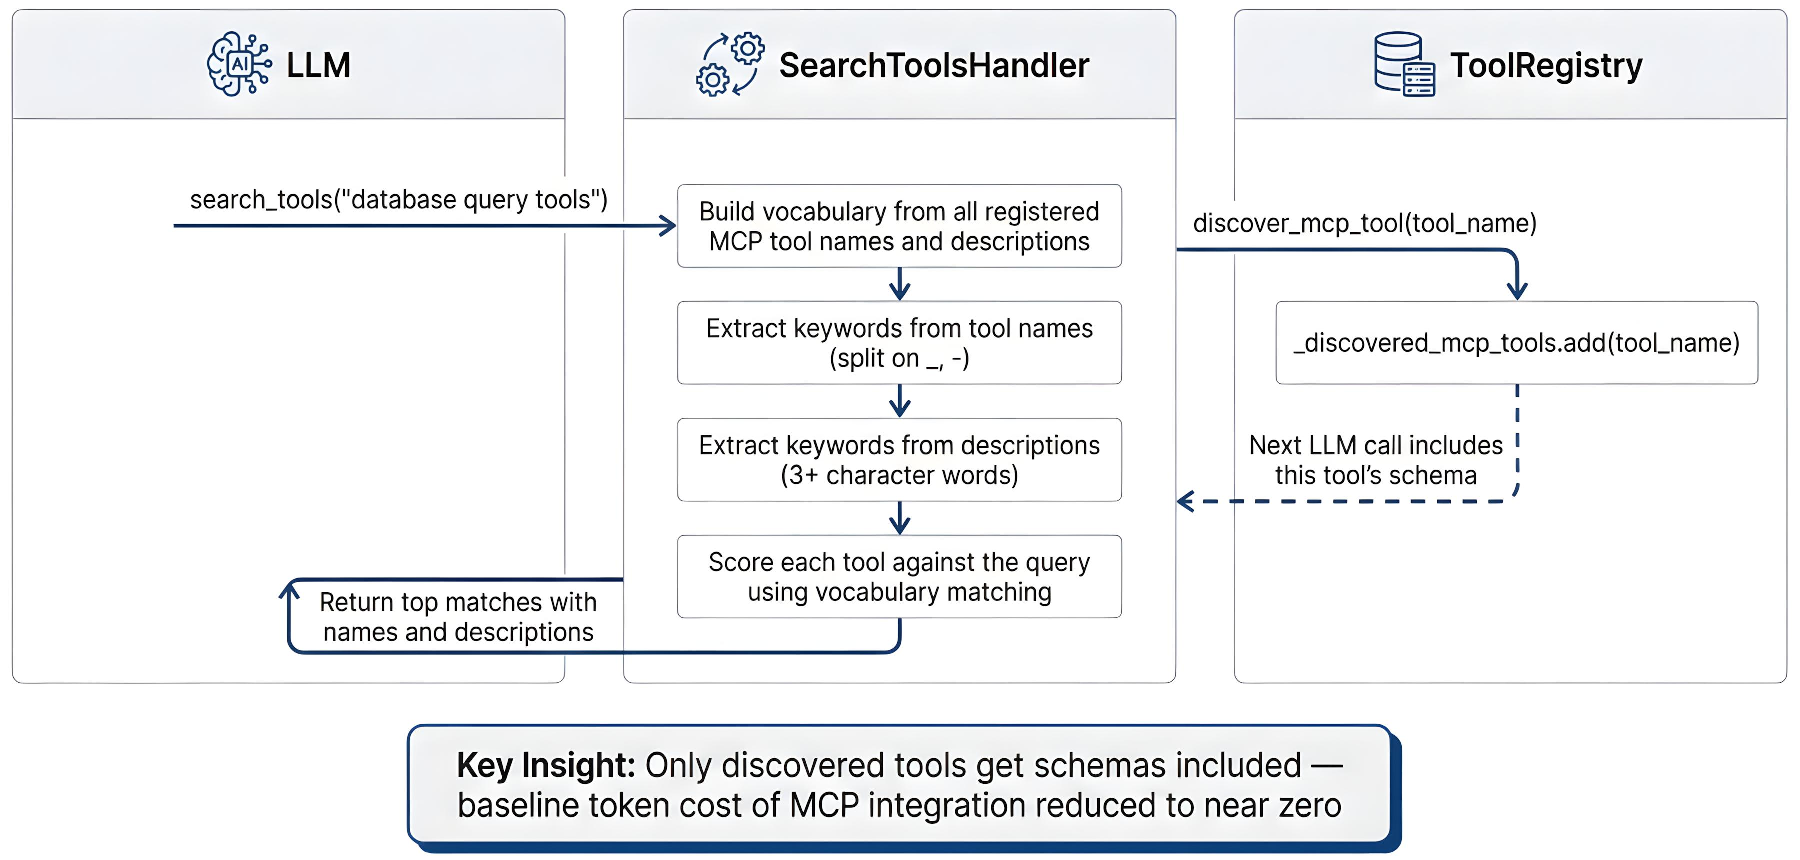
\includegraphics[width=\linewidth]{figures/token_efficient_mcp_discovery.pdf}
    \caption{Sequence within the Tool layer (\Cref{fig:tool_system}). The LLM issues a \texttt{search\_tools} call with a natural-language query. The \texttt{SearchToolsHandler} builds a keyword vocabulary from all registered MCP tool names and descriptions, scores each tool against the query, and returns top matches. The \texttt{ToolRegistry} marks matched tools as discovered, including their schemas in subsequent LLM calls. Only discovered tools incur schema cost, reducing baseline token overhead of MCP integration to near zero.}
    \label{fig:mcp_discovery}
\end{figure}

\paragraph{\texttt{search\_tools}: Keyword-scored tool discovery.} Three detail levels control context investment: \texttt{names} returns only tool names (minimal tokens), \texttt{brief} adds short descriptions, and \texttt{full} triggers full schema inclusion in subsequent LLM calls. Name matches score 2 points and description matches score 1 point; results rank by total score, surfacing the most relevant tools first. This trades discovery overhead (the agent must search, then invoke) for context savings (only relevant tools are loaded). For workflows using few external tools, the savings are substantial; for workflows using many, the overhead accumulates but remains bounded.

\paragraph{Design evolution.} The initial implementation included all external tool schemas in every call, consuming up to 40\% of the context before the first user message. Lazy discovery reduced baseline overhead to nearly zero ($<$5\%), growing only as capabilities are actually used.

\subsubsection{Subagent Delegation, Skills, and Batch Execution}
\label{sec:tools_advanced}

This section describes three tools that extend the agent's capabilities beyond single-tool invocations: subagent delegation for complex subtasks, skill loading for on-demand domain expertise, and batch execution for multi-tool efficiency.

\paragraph{Subagent delegation via \texttt{spawn\_subagent}.} Launches an isolated subagent with its own ReAct loop and filtered tool registry. Each of the eight subagent types restricts available tools to its domain: Code-Explorer (read-only navigation), Planner (read + write for plans), PR-Reviewer (code review with diff analysis), Security-Reviewer (vulnerability scanning), Web-Clone (website replication), Web-Generator (site creation from specifications), Project-Init (scaffold generation), and Ask-User (UI-only structured surveys). The tool isolation ensures subagents cannot accidentally interfere with each other or exceed their intended scope. \Cref{app:subagents} provides the complete capability matrix with per-subagent tool lists.

A key design property is automatic parallelization: when the main agent emits multiple \texttt{spawn\_subagent} calls in the same LLM response, the \texttt{SubAgentManager} executes them concurrently via \texttt{asyncio.gather()}, with each subagent running in a separate thread with its own iteration budget and tool worker pool. This enables the agent to fan out work naturally (e.g., ``investigate the authentication module'' and ``review the database schema'' in parallel) without explicit concurrency management.

Additional parameters provide flexibility: model override (haiku for fast, low-cost tasks; sonnet for balanced capability; opus for complex reasoning), background execution (agent continues without waiting for completion), and session resume by agent ID (enabling multi-turn subagent workflows where context is preserved across invocations).

\paragraph{On-demand skills via \texttt{invoke\_skill}.} Skills are modular knowledge units stored as markdown files with YAML frontmatter, providing domain-specific expertise (git conventions, code review checklists, deployment procedures) that would waste context if loaded unconditionally. The system processes skills in two phases:

\textbf{Phase~1: Metadata discovery.} At startup, the \texttt{SkillLoader} scans all skill directories, parsing only the YAML frontmatter to extract names and descriptions. This lightweight index is included in the system prompt, enabling the agent to discover available expertise without loading instructional content. Descriptions follow a ``Claude Search Optimization'' convention where each begins with ``Use when\ldots'' to specify trigger conditions (e.g., ``Use when writing bash scripts that need to wait for external conditions''), optimizing for agent discoverability.

\textbf{Phase~2: On-demand loading.} When the agent determines a skill is relevant, it invokes \texttt{invoke\_skill} with the skill name. The loader reads the full markdown content, strips the frontmatter, and injects the instructional body into the conversation context. A deduplication cache ensures each skill loads at most once per session, preventing context pollution from redundant invocations.

Skills are discovered from three tiers with strict priority ordering: project-local (\texttt{.opendev/skills/}, highest priority) for repository-specific conventions, user-global (\texttt{\~{}/.opendev/skills/}) for personal preferences across all projects, and built-in (shipped with the package, lowest priority) for default expertise. When two skills share the same name, the higher-priority source takes precedence, enabling project-specific overrides of default behavior.

\paragraph{Batch execution via \texttt{batch\_tool}.} Enables multiple tool calls in a single agent turn, reducing round-trip overhead. The agent specifies the execution mode: \emph{parallel} (thread pool with max 5 concurrent workers) for independent operations like reading multiple files or running multiple searches, or \emph{serial} for dependent operations like creating a directory then writing a file into it. The agent specifies the mode because only it knows the dependency relationships from context, as the system cannot reliably infer whether operations are independent. Automatic dependency detection was attempted but proved unreliable; explicit agent-specified mode delegating the decision to the entity with full context knowledge solved this cleanly.

\paragraph{Design evolution.} The initial design had no batch execution; every tool required a full LLM round-trip, and multiple file reads took multiple turns. Skills were originally loaded at startup, consuming context on expertise never used in the session. Subagents initially ran sequentially, even when tasks were independent. The current architecture addresses all three issues: batch execution eliminates unnecessary round-trips, two-phase skill loading reduces baseline overhead to a compact metadata index, and automatic parallelization of subagent calls exploits task independence without requiring the agent to manage concurrency explicitly.
